\section{Transaction Management}

\subsection{Introduction}

In the previous section, we focused on queries used to access the DB with the purpose of reading data (optimization, data movement, indices). In this section, we focus on transactions. Transactions are accesses to the DB with the purpose of modifying the data (update, insert, delete). Important is: correctness, recovery and state management.

Concurrency control and recovery are deeply interrelated. CC implementation affects recovery implementation and recovery implementation restricts what can be done in terms of CC.

\begin{figure}[h]
	\centering
	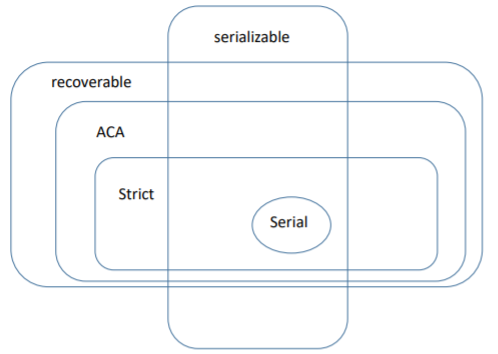
\includegraphics[scale=0.6]{images/4-histories.PNG}
	\caption{Consistency and recoverability properties.}
	\label{fig:histories}
\end{figure}




\subsection{Transaction Model}

\paragraph{Transaction}
A unit of work made up of multiple operations (read and / or write) that has all the properties specified by ACID - operations inside the same transaction cannot be reordered. A transaction can either commit, i.e. its changes are made persistent, or abort / rollback, i.e. it is cancelled and all changes are reverted. Some systems include the concept of a savepoint, i.e. temporarily committing changes until a certain point with the possibility of rollback to a savepoint.

\paragraph{Transaction Manager}
Enforces concurrency control in a DB engine. It includes (see Figure \ref{fig:manager}):
\begin{itemize}
    \item \textbf{Transaction Table:} List (commonly in common area) of active transactions in the system.
    \item \textbf{Transaction Handler:} Pointer to the structures containing all the relevant info related to a transaction (possibly in private area).
    \item \textbf{Lock Table:} Hash table containing entries that correspond to active locks. Locks on the same item = linked list.
    \item \textbf{Log:} Entries that capture the operations performed and are kept in memory until they're written back to disk.
\end{itemize}
A transaction manager goes through the following operations:
\begin{itemize}
    \item \textbf{Begin T:} Create entry in transaction table (no log entry unless explicitly requested).
    \item \textbf{Read/Write:} Hash tuple ID to find corresponding entry in lock table. If empty: grant lock to T, else: attach request to list and grant request if compatible.
    \item \textbf{Write:} Create log entry (with LSN, before/after image, transaction ID, pointers to previous log entry of same T, etc.).
    \item \textbf{Commit T:} Release lock, potentially resume transactions waiting for lock, finalize log entries, write log entries to storage, potentially write modified data to storage, etc.
    \item \textbf{Abort T:} Release lock, potentially resume transactions waiting for lock, use log entries to undo/discard changes, potentially write log entries to storage, etc.
\end{itemize}

\begin{figure}[h]
	\centering
	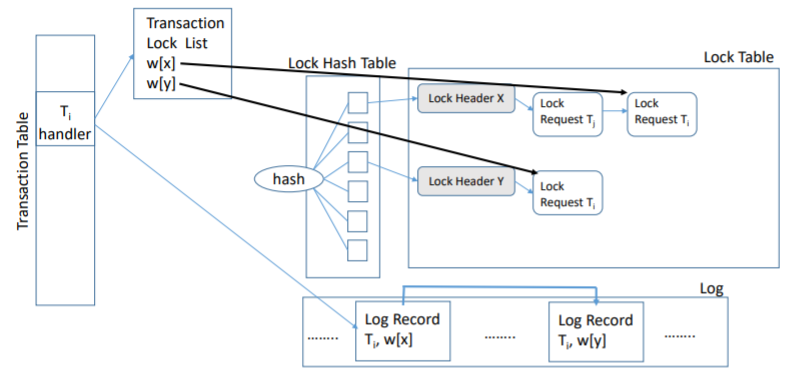
\includegraphics[scale=0.7]{images/4-manager.PNG}
	\caption{Basic functions of a transaction manager.}
	\label{fig:manager}
\end{figure}

%TODO more on lock table? other trans. manager designs

\paragraph{Conflicts}
\begin{itemize}
    \item \textbf{Write-Read (WR) / Dirty Read:} T2 reads object modified by T1 before T1 committed.
    \item \textbf{Read-Write (RW) / Unrepeatable Read:} T1 reads object that is modified and committed by T2, T1 then reads the same object again which results in a different value.
    \item \textbf{Write-Write (WW) / Lost Update:} T1 modifies an object previously modified by T2 with T1 committing before T2.
\end{itemize} 
If no write is involved, read-read (RR) does not cause a conflict.

%TODO abort / commit conflicts

\paragraph{History / Schedule} %SUMMARY image, serial vs. recover
A partially ordered sequence of operations from a set of transactions. 



\subsection{Concurrency Control}

How to ensure that the data remains consistent (data integrity) with a number of transactions and queries running at the same time.

\paragraph{ACID}
A set of properties of transactions intended to guarantee data validity despite errors, power failures and other mishaps. See Figure \ref{fig:acid}.

\textbf{Atomicity:} (Group of) operations taking place in their entirety or not at all. Intermediate states are not guaranteed to be correct. Atomicity requires isolation meaning that intermediate state should never be seen by another transaction.

\textbf{Consistency:} Assumption that an accepted transaction is correct (according to all defined rules / constraints).

\textbf{Isolation:} Property defining how / when the changes made by one operation become visible to others. Usually, transactions will be executed as if they were alone (intermediate state is not visible). Isolation is enforced with locking mechanisms.

\textbf{Durability:} Guarantee that transactions that have committed will survive permanently. Usually handled with some kind of logging mechanism, i.e. capturing consistent states in snapshots.

\paragraph{Serial History}
A history is serial if for every two transactions that appear in it either all operations of the first one appear before all operations of the second one or vice versa. By definition, a serial history with only committed transactions is correct (isolation, transactions start and end in a consistent state).

\paragraph{Equivalent Histories}
Two histories are equivalent iff they include the same transactions containing the same operations and conflicting operations of non-aborted transactions are ordered the same way in both histories. This implies that committed transactions in either history see the same state and leave the DB in the same state (same effects).

\paragraph{Conflict Equivalent Histories}
One can be transformed to the other by swapping non-conflicting operations.

\paragraph{Serializable History}
History is serializable iff it is equivalent to a serial history. If it is, it is correct (leaves the DB in a consistent state). %TODO commit included?

\paragraph{Serializability Graph}
A compact representation of the dependencies in a history. One node per committed transaction. Edge from T to T' if an action of T precedes and is in conflict with an action of T'. %TODO examples

\paragraph{Serializability Theorem}
A history is serializable iff its serializability graph is acyclic. Sorting it topologically results in an equivalent serial history.

\paragraph{Conflict Serializability}
If a history can be transformed into a serial history by swapping non-conflicting operations it is conflict serializable.



\subsection{Recovery}

How to ensure that the data remains consistent even when unexpected failures occur. A.k.a. changes from transactions that have not completed are not visible and changes from committed transactions are recorded and visible.

\paragraph{Types of Failures}
\begin{itemize}
    \item Transaction failure (abort, fail, time out, etc.) - undo its changes.
    \item System failure - bring DB back to a consistent state (undo and redo).
    \item Media failure (disk fail, permanent storage has errors, etc.) - restore DB to a known consistent state (replication, separating data from log files, etc.).
\end{itemize}

\paragraph{Recovery Procedures}
\begin{itemize}
    \item \textbf{R1:} Undo all changes from a single transaction - regardless of why.
    \item \textbf{R2:} Redo changes from committed transactions in case of a system crash where main memory is lost and disk is kept.
    \item \textbf{R3:} Undo the changes that remain in the system from active transactions in case of a system crash where main memory is lost and disk is kept.
    \item \textbf{R4:} Read consistent snapshots from backup and if possible apply the log (in case of system crash with loss of disk).
\end{itemize}

\paragraph{Undo vs. Redo}
To ensure atomicity in case of a non-completed transaction, we either need to: restore the initial DB state and remove any effects of the transaction (before image) or reach the intended final state of the transaction in question. Redo might also be applied to restore the changes of already committed transactions (after image).

\paragraph{Recoverable History (RC)}
If T2 reads an object modified by T1 and commits, T1 committed before T2 did. A committed transaction does not need to be undone since it cannot read wrong data and transactions commit in their serialization order.

\paragraph{Avoids Cascading Abort History (ACA)}
If T2 reads an object modified by T1, the read has happened after T2 committed. Aborting a transaction does not cause aborting others and transactions only read from committed transactions.

\paragraph{Strict History (ST)}
If T2 reads / writes an object modified by T1, the operation has happened after T2 committed or aborted. Undoing a transaction does not undo the changes of other transactions and transactions do not read / write updates of uncommitted transactions.

\paragraph{SQL Isolation Levels (ANSI)}
%TODO

\paragraph{Logging}
In case of system failure (sudden loss of data in memory) the engine needs to recover the DB up to the point of its last committed state which includes all changes made by all committed transactions up until time of failure = recovery procedure. The recovery procedure can only operate with data on permanent storage and needs to be correct even if successive failures occur in the middle of it. To do this, we need to be able to do logging.

%TODO serial. strict p6? when to write undo redo shit

\paragraph{Recovery Procedure}
A recovery procedure implemented by a recovery manager requires either undo and redo, just undo or just redo or neither. Undo needs before images (write back before commit) and redo needs after images (write back after commit). %TODO steal and force

\paragraph{Undo and Redo}
\begin{itemize}
    \item \textbf{Read:} Simply read value from block on buffer cache.
    \item \textbf{Write:} Create log entry (before and after image) and append to persistent log. Write after image to block on buffer cache.
    \item \textbf{Commit:} Write persistent log entry indicating that T has committed.
    \item \textbf{Abort:} For all updates, restore the before image using the log entry.
\end{itemize}
The recovery procedure will start from the end of the log and work backwards and keep two lists: undone items and redone items. Procedure terminates when all items are in either list or we're at the beginning of the log. For each log entry: if the accessed item is not yet in a list apply after image and add to redone list if it is part of a committed T or apply before image and add to undone list if it is part of an aborted T. %TODO pros

\paragraph{Just Undo}
\begin{itemize}
    \item \textbf{Read:} Simply read value from block on buffer cache.
    \item \textbf{Write:} Create log entry (before image) and append to persistent log. Write after image to block on buffer cache.
    \item \textbf{Commit:} Flush all dirty values modified by T if still in cache. Write persistent log entry indicating that T has committed.
    \item \textbf{Abort:} For all updates, restore the before image using the log entry.
\end{itemize}
Procedure same as above just with one undone list - each item part of an aborted T is restored to before image and added to this list. This relies on the fact that all committed values are in persistent storage and have not been lost. Works if strict execution is assumed. %TODO comments

\paragraph{Just Redo}
\begin{itemize}
    \item \textbf{Read:} If T has not written value before, read it from buffer cache. Else: read value from temporary buffer.
    \item \textbf{Write:} Create log entry (after image) and append to persistent log. Write after image to some temporary buffer.
    \item \textbf{Commit:} Apply all updates in temporary buffer to actual data blocks. Write persistent log entry indicating that T has committed.
    \item \textbf{Abort:} Discard temporary buffer.
\end{itemize}
Procedure same as above just with one redone list - each item not in list and part of a committed T is added to list and changes are redone using before image. Relies on never having dirty blocks in buffer cache - all data there is committed and is the most recent version. %TODO comments

\paragraph{Neither}
Rare resp. not used in practice, does not require a log and also there is no recovery procedure (that's the point). Uncommitted data is never written to persistent storage and data in memory is never dirty. Requires ability to write all changes made by a transaction to persistent storage in a single atomic action. %TODO data structures
\begin{itemize}
    \item \textbf{Read:} If T has not written value before, use current directory to find latest committed copy. Else: use shadow directory of T to find updated copy.
    \item \textbf{Write:} Write to buffer and add pointer to shadow directory of T.
    \item \textbf{Commit:} Create full directory by merging current one and shadow one of T. Swap pointer indicating latest committed directory.
    \item \textbf{Abort:} Discard buffer and shadow directory.
\end{itemize} %TODO comments

\paragraph{Log Record}
Log sequence number (LSN) for navigation, system change number (SCN) for event timestamps (T start), pointers to other log records of same T, transaction ID and related info (redo: change vectors = after images - describes changes to single block of data, undo: before images).
%TODO log blocks. more on SCN

\textbf{In Memory:} %TODO
\textbf{In Storage:} %TODO

%TODO




\subsection{Locking}

Concurrency control in DBs is implemented using locking (usually with a lock table as seen in a transaction manager).

\paragraph{Compatibility Matrix}
%TODO lock modes? granularity stuff

\paragraph{Two Phase Locking (2PL)}

\paragraph{Strict 2PL}

\paragraph{Deadlock Detection}

\paragraph{Snapshot Isolation}







\subsection{Reading Assignments}

\subsubsection{Concurrency Control and Recovery in Database Systems}

\subsection{Exercises}

\subsubsection{Serializability and 2PL}

\subsubsection{Recovery}